\chapter*{Typesetting}%
\label{ch:typesetting}

\section*{Text Formatting}%
\label{sec:text-formatting}

\subsection*{Bold, Italic, Underlining and Emphasis}%
\label{subsec:bold-italic-underlining-and-emphasis}

\begin{lstlisting}[caption={Bold, italic, underlining and emphasis.}]
\textbf{Lorem ipsum} \underline{dolor} sit amet, \textit{consectetur}
\textbf{\textit{adipiscing elit}, sed do eiusmod \textbf{tempor incididunt
ut labore et \emph{dolore} magna aliqua}.
\end{lstlisting}

\textbf{Lorem ipsum} \underline{dolor} sit amet, \textit{consectetur}
\textbf{\textit{adipiscing elit}}, sed do eiusmod \textbf{tempor incididunt
ut labore et \emph{dolore} magna aliqua}.

\subsection*{Paragraphs, New Lines and Text Justification}%
\label{subsec:paragraphs-new-lines-and-text-justification}

\begin{lstlisting}[caption={Paragraphs, new lines and text justification.}]
``Lorem ipsum dolor sit amet, consectetur adipiscing elit,
sed do eiusmod tempor incididunt ut labore et dolore magna aliqua.''

\begin{flushleft}
Ut enim ad minim veniam, quis nostrud exercitation ullamco laboris nisi ut
aliquip ex ea commodo consequat. Duis aute irure dolor in reprehenderit in
voluptate velit esse cillum dolore eu fugiat nulla pariatur.
\end{flushleft}

\begin{center}
Excepteur sint occaecat cupidatat non proident, sunt in culpa qui officia
deserunt mollit anim id est laborum.
\end{center}

\begin{flushright}
Sed ut perspiciatis unde omnis iste natus error sit voluptatem accusantium
doloremque laudantium, totam rem aperiam, eaque ipsa quae ab illo inventore
veritatis et quasi architecto beatae vitae dicta sunt explicabo.
\end{flushright}

Nemo enim ipsam voluptatem quia voluptas sit aspernatur aut odit aut fugit,
sed quia consequuntur magni dolores eos qui ratione voluptatem sequi nesciunt.
\ccPar{}
Neque porro quisquam est, qui dolorem ipsum quia dolor sit amet, consectetur,
adipisci velit, sed quia non numquam eius modi tempora incidunt ut labore et
dolore magnam aliquam quaerat voluptatem.
\ccPar{}
Ut enim ad minima veniam, quis nostrum exercitationem ullam corporis suscipit
laboriosam, nisi ut aliquid ex ea commodi consequatur?
\end{lstlisting}

``Lorem ipsum dolor sit amet, consectetur adipiscing elit,
sed do eiusmod tempor incididunt ut labore et dolore magna aliqua.''

\begin{flushleft}
Ut enim ad minim veniam, quis nostrud exercitation ullamco laboris nisi ut
aliquip ex ea commodo consequat. Duis aute irure dolor in reprehenderit in
voluptate velit esse cillum dolore eu fugiat nulla pariatur.
\end{flushleft}

\begin{center}
Excepteur sint occaecat cupidatat non proident, sunt in culpa qui officia
deserunt mollit anim id est laborum.
\end{center}

\begin{flushright}
Sed ut perspiciatis unde omnis iste natus error sit voluptatem accusantium
doloremque laudantium, totam rem aperiam, eaque ipsa quae ab illo inventore
veritatis et quasi architecto beatae vitae dicta sunt explicabo.
\end{flushright}

Nemo enim ipsam voluptatem quia voluptas sit aspernatur aut odit aut fugit,
sed quia consequuntur magni dolores eos qui ratione voluptatem sequi nesciunt.
\ccPar{}
Neque porro quisquam est, qui dolorem ipsum quia dolor sit amet, consectetur,
adipisci velit, sed quia non numquam eius modi tempora incidunt ut labore et
dolore magnam aliquam quaerat voluptatem.
\ccPar{}
Ut enim ad minima veniam, quis nostrum exercitationem ullam corporis suscipit
laboriosam, nisi ut aliquid ex ea commodi consequatur?

\section*{Footnotes}%
\label{sec:footnotes}

\begin{lstlisting}[caption={Some footnotes.}]
Lorem ipsum dolor sit amet, consectetur adipiscing elit\footnote{Ut enim ad
minim veniam, quis nostrud exercitation ullamco laboris nisi ut aliquip ex ea
commodo consequat. Duis aute irure dolor in reprehenderit in voluptate velit
esse cillum dolore eu fugiat nulla pariatur.}, sed do eiusmod tempor incididunt
ut labore et dolore magna aliqua.

\begin{center}
Excepteur sint occaecat cupidatat non proident, sunt in culpa qui officia
deserunt mollit anim id est laborum.\footnote{Sed ut perspiciatis unde omnis
iste natus error sit voluptatem accusantium doloremque laudantium, totam rem
aperiam, eaque ipsa quae ab illo inventore veritatis et quasi architecto
beatae vitae dicta sunt explicabo.}
\end{center}
\end{lstlisting}

Lorem ipsum dolor sit amet, consectetur adipiscing elit\footnote{Ut enim ad
minim veniam, quis nostrud exercitation ullamco laboris nisi ut aliquip ex ea
commodo consequat. Duis aute irure dolor in reprehenderit in voluptate velit
esse cillum dolore eu fugiat nulla pariatur.}, sed do eiusmod tempor incididunt
ut labore et dolore magna aliqua.

\begin{center}
Excepteur sint occaecat cupidatat non proident, sunt in culpa qui officia
deserunt mollit anim id est laborum.\footnote{Sed ut perspiciatis unde omnis
iste natus error sit voluptatem accusantium doloremque laudantium, totam rem
aperiam, eaque ipsa quae ab illo inventore veritatis et quasi architecto
beatae vitae dicta sunt explicabo.}
\end{center}

\section*{Quotations}%
\label{sec:quotations}

\subsection*{Basic Quotation}%
\label{subsec:basic-quotation}

\begin{lstlisting}[caption={Basic quotation.}]
At vero eos:~\blockquote{et accusamus et iusto odio dignissimos ducimus qui
blanditiis praesentium voluptatum deleniti atque corrupti quos dolores et quas
molestias excepturi sint occaecati cupiditate non provident}
\end{lstlisting}

At vero eos:~\blockquote{et accusamus et iusto odio dignissimos ducimus qui
blanditiis praesentium voluptatum deleniti atque corrupti quos dolores et quas
molestias excepturi sint occaecati cupiditate non provident}

\subsection*{Quotation with Citation}%
\label{subsec:quotation-with-citation}

\begin{lstlisting}[caption={Quotation with Citation.}]
Mark D. Fairchild writes:~\blockcquote[85]{Fairchild2013u}{Almost everyone
knows what color is. After all, they have had firsthand experience of it since
shortly after birth. However, very few can precisely describe their color
experiences or even precisely define color.}
\end{lstlisting}

Mark D. Fairchild writes:~\blockcquote[85]{Fairchild2013u}{Almost everyone
knows what color is. After all, they have had firsthand experience of it since
shortly after birth. However, very few can precisely describe their color
experiences or even precisely define color.}

\section*{Key Points and Concepts Review}%
\label{sec:key-points-and-concepts-review}

\begin{lstlisting}[caption={Key points and concepts review.}]
\begin{ccKeyPoints}
    \begin{itemize}
        \item Color science studies the human perception of color,
its measurement, and characterization.
        \item Proper terminology usage is critical to the understanding of a
scientific field.
        \item Color is the characteristic of a visual perception.
        \item Color management depends on colorimetry, the measurement of color.
    \end{itemize}
\end{ccKeyPoints}
\end{lstlisting}

\begin{ccKeyPoints}
    \begin{itemize}
        \item Color science studies the human perception of color,
its measurement, and characterization.
        \item Proper terminology usage is critical to the understanding of a
scientific field.
        \item Color is the characteristic of a visual perception.
        \item Color management depends on colorimetry, the measurement of color.
    \end{itemize}
\end{ccKeyPoints}

\section*{Hyperlinks}%
\label{sec:hyperlinks}

\begin{lstlisting}[caption={Hyperlinks.}]
Some links to Equations~\ref{eq:e-mc2},~\ref{eq:a-fracpir22}, and~\ref{eq:2x5y-8}.

A link to Table~\ref{tab:a-table-with-mathematics}.

Some links to Figures~\ref{fig:wir2-ralph-mapped-to-709} and~\ref{fig:aces-gamuts}.

A link to Chapter~\ref{ch:introduction}.

A link to Section~\ref{sec:intended-audience}.

A link to Section~\ref{subsec:open-source-software}.

A link to Section~\ref{subsubsec:abney-effect}.

A named link to Section~\nameref{subsubsec:abney-effect}.

An achromatic named link to~\ccAchromaticNameref{subsubsec:abney-effect} section.
\end{lstlisting}

Some links to Equations~\ref{eq:e-mc2},~\ref{eq:a-fracpir22}, and~\ref{eq:2x5y-8}.

A link to Table~\ref{tab:a-table-with-mathematics}.

Some links to Figures~\ref{fig:wir2-ralph-mapped-to-709} and~\ref{fig:aces-gamuts}.

A link to Chapter~\ref{ch:introduction}.

A link to Section~\ref{sec:intended-audience}.

A link to Section~\ref{subsec:open-source-software}.

A link to Section~\ref{subsubsec:abney-effect}.

A named link to Section~\nameref{subsubsec:abney-effect}.

An achromatic named link to~\ccAchromaticNameref{subsubsec:abney-effect} section.

\section*{Lists}%
\label{sec:lists}

\subsection*{Unordered List}%
\label{subsec:unordered-list}

\begin{lstlisting}[caption={An unordered list.}]
\begin{itemize}
    \item First item of first level.
    \item Second item of first level.
    \item Third item of first level.
\end{itemize}
\end{lstlisting}

\begin{itemize}
    \item First item of first level.
    \item Second item of first level.
    \item Third item of first level.
\end{itemize}

\subsection*{Ordered List}%
\label{subsec:ordered-list}

\begin{lstlisting}[caption={An ordered list.}]
\begin{enumerate}
    \item First item of first level.
    \item Second item of first level.
    \item Third item of first level.
\end{enumerate}
\end{lstlisting}

\begin{enumerate}
    \item First item of first level.
    \item Second item of first level.
    \item Third item of first level.
\end{enumerate}

\subsection*{Nested List}%
\label{subsec:nested-list}

\begin{lstlisting}[caption={A nested list.}]
\item First item of first level.
\begin{itemize}
    \item First item of second level.
    \item Second item of second level.
    \item Third item of second level.
\end{itemize}
\item Second item of first level.
\item Third item of first level.
\end{lstlisting}

\begin{enumerate}
    \item First item of first level.
    \begin{itemize}
        \item First item of second level.
        \item Second item of second level.
        \item Third item of second level.
    \end{itemize}
    \item Second item of first level.
    \item Third item of first level.
\end{enumerate}

\section*{Tables}%
\label{sec:tables}

\subsection*{Table with Mathematics}%
\label{subsec:table-with-mathematics}

\begin{lstlisting}[caption={A table with mathematics.}]
\begin{table}[H]
    \begin{tabular}{l c c c c c c c c c c c}
        \ccLatexHLine
        $\boldsymbol{EV}$ & -8 & -3 & -2 & -1 & -0.5 & 0 & 0.5 & 1 & 2 & 3 & 8 \\
        \ccLatexHLine
        $\boldsymbol{2^{EV}}$ & 0.004 & 0.125 & 0.25 & 0.5 & 0.707 & 1 & 1.414 & 2 & 4 & 8 & 256 \ccLatexNewline
        \ccLatexHLine
    \end{tabular}
    \caption{A table with mathematics.}
    \label{tab:a-table-with-mathematics}
\end{table}
\end{lstlisting}

\begin{table}[H]
    \begin{tabular}{l c c c c c c c c c c c}
        \ccLatexHLine
        $\boldsymbol{EV}$ & -8 & -3 & -2 & -1 & -0.5 & 0 & 0.5 & 1 & 2 & 3 & 8 \\
        \ccLatexHLine
        $\boldsymbol{2^{EV}}$ & 0.004 & 0.125 & 0.25 & 0.5 & 0.707 & 1 & 1.414 & 2 & 4 & 8 & 256 \ccLatexNewline
        \ccLatexHLine
    \end{tabular}
    \caption{A table with mathematics.}
    \label{tab:a-table-with-mathematics}
\end{table}

\section*{Mathematics}%
\label{sec:mathematics}

\subsection*{Inline Mathematics}%
\label{subsec:inline-mathematics}

\begin{lstlisting}[caption={Inline mathematics.}]
The well known Pythagorean theorem \(x^2 + y^2 = z^2\) was
proved to be invalid for other exponents.
Meaning the next equation has no integer solutions:

\[ x^n + y^n = z^n \]
\end{lstlisting}

The well known Pythagorean theorem \(x^2 + y^2 = z^2\) was
proved to be invalid for other exponents.
Meaning the next equation has no integer solutions:

\[x^n + y^n = z^n\]

\subsection*{Equations}%
\label{subsec:equations}

\begin{lstlisting}[caption={Equations.}]
\begin{equation}
    E=mc^2
    \label{eq:e-mc2}
\end{equation}

\begin{equation}
    \begin{split}
        A & = \frac{\pi r^2}{2} \\
          & = \frac{1}{2} \pi r^2
    \end{split}
    \label{eq:a-fracpir22}
\end{equation}

\begin{align}
    2x - 5y & =  8 \\
    3x + 9y & =  -12
    \label{eq:2x5y-8}
\end{align}
\end{lstlisting}

\begin{equation}
    E=mc^2
    \label{eq:e-mc2}
\end{equation}

\begin{equation}
    \begin{split}
        A & = \frac{\pi r^2}{2} \\
          & = \frac{1}{2} \pi r^2
    \end{split}
    \label{eq:a-fracpir22}
\end{equation}

\begin{align}
    2x - 5y & =  8 \\
    3x + 9y & =  -12
    \label{eq:2x5y-8}
\end{align}

\section*{Figures and Images}%
\label{sec:figures-and-images}

To ensure that both \textit{PDF} and \textit{HTML} output are embedding
``JPG'' images, ``JPG'' paths must be given with their extensions.

\subsection*{``JPG'' Raster File}%
\label{subsec:jpg-raster-file}

\begin{lstlisting}[caption={Embedding a ``JPG'' raster file.}]
\begin{figure}[H]
    
\includegraphics[alt={RBI - Ralph mapped to Rec.709.},width=\textwidth]{wir2-ralph-mapped-to-709.jpg}
    \caption{
        Lorem ipsum dolor sit amet, consectetur adipiscing elit,
        sed do eiusmod tempor incididunt ut labore et dolore magna aliqua.
    }
    \label{fig:wir2-ralph-mapped-to-709}
\end{figure}
\end{lstlisting}

\begin{figure}[H]
    
\includegraphics[alt={RBI - Ralph mapped to Rec.709.},width=\textwidth]{wir2-ralph-mapped-to-709.jpg}
    \caption{
        Lorem ipsum dolor sit amet, consectetur adipiscing elit,
        sed do eiusmod tempor incididunt ut labore et dolore magna aliqua.
    }
    \label{fig:wir2-ralph-mapped-to-709}
\end{figure}

\subsection*{``SVG'' Vector File}%
\label{subsec:svg-vector-file}

\begin{lstlisting}[caption={Embedding a ``SVG'' vector file.}]
\begin{figure}[H]
    \includesvg[alt={ACES - Gamuts},width=\textwidth]{aces-gamuts}
    \caption{
        Lorem ipsum dolor sit amet, consectetur adipiscing elit,
        sed do eiusmod tempor incididunt ut labore et dolore magna aliqua.
    }
    \label{fig:aces-gamuts}
\end{figure}
\end{lstlisting}

\begin{figure}[H]
    \includesvg[alt={ACES - Gamuts},width=\textwidth]{aces-gamuts}
    \caption{
        Lorem ipsum dolor sit amet, consectetur adipiscing elit,
        sed do eiusmod tempor incididunt ut labore et dolore magna aliqua.
    }
    \label{fig:aces-gamuts}
\end{figure}

\subsection*{Simple Jeri Embedding}%

A simple \textit{Jeri} embedding example that shows in both the \textit{HTML}
and \textit{PDF} outputs.

\begin{lstlisting}[caption={Simple \textit{Jeri} Embedding.}]
\begin{figure}[H]
    \unless\ifdefined\HCode
        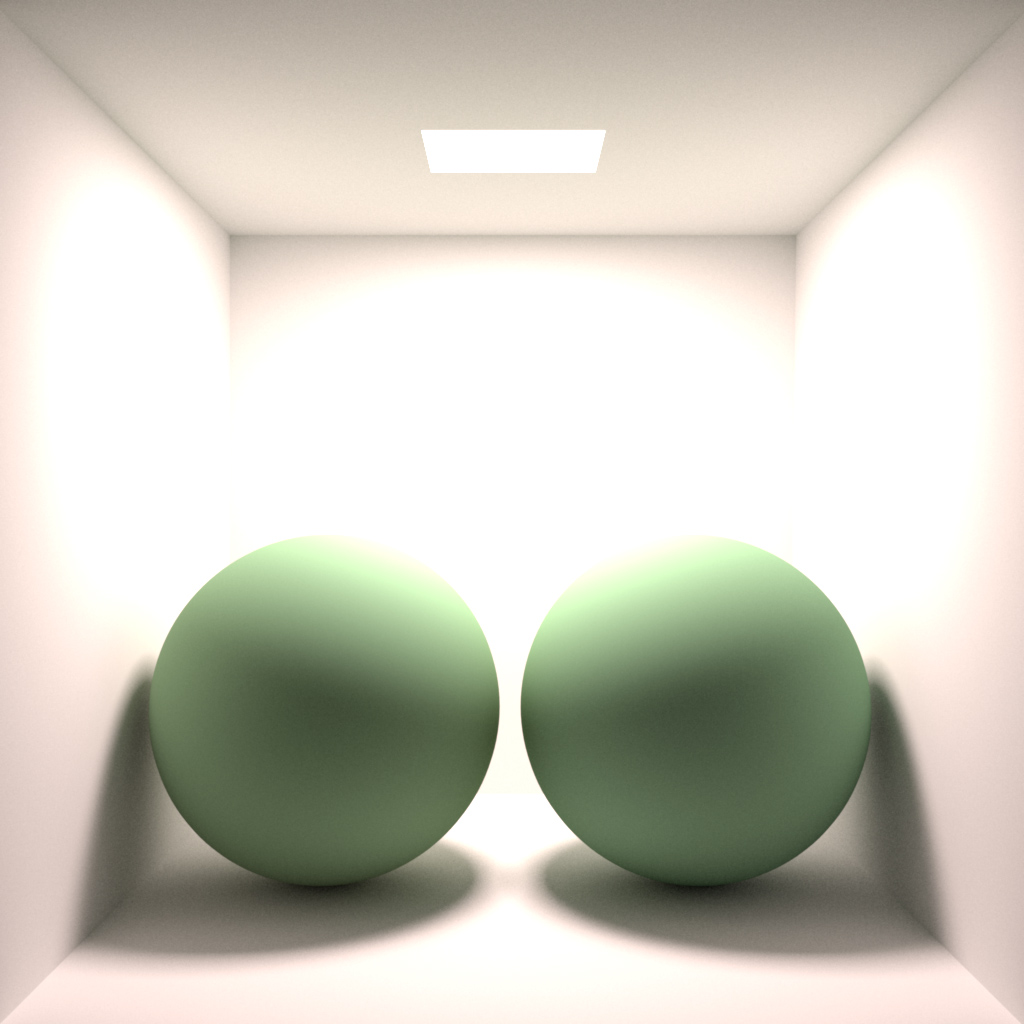
\includegraphics[alt={Illuminant E.},width=0.475\textwidth]{mitsuba-cornellbox-metamerism-E.jpg}\hfill
        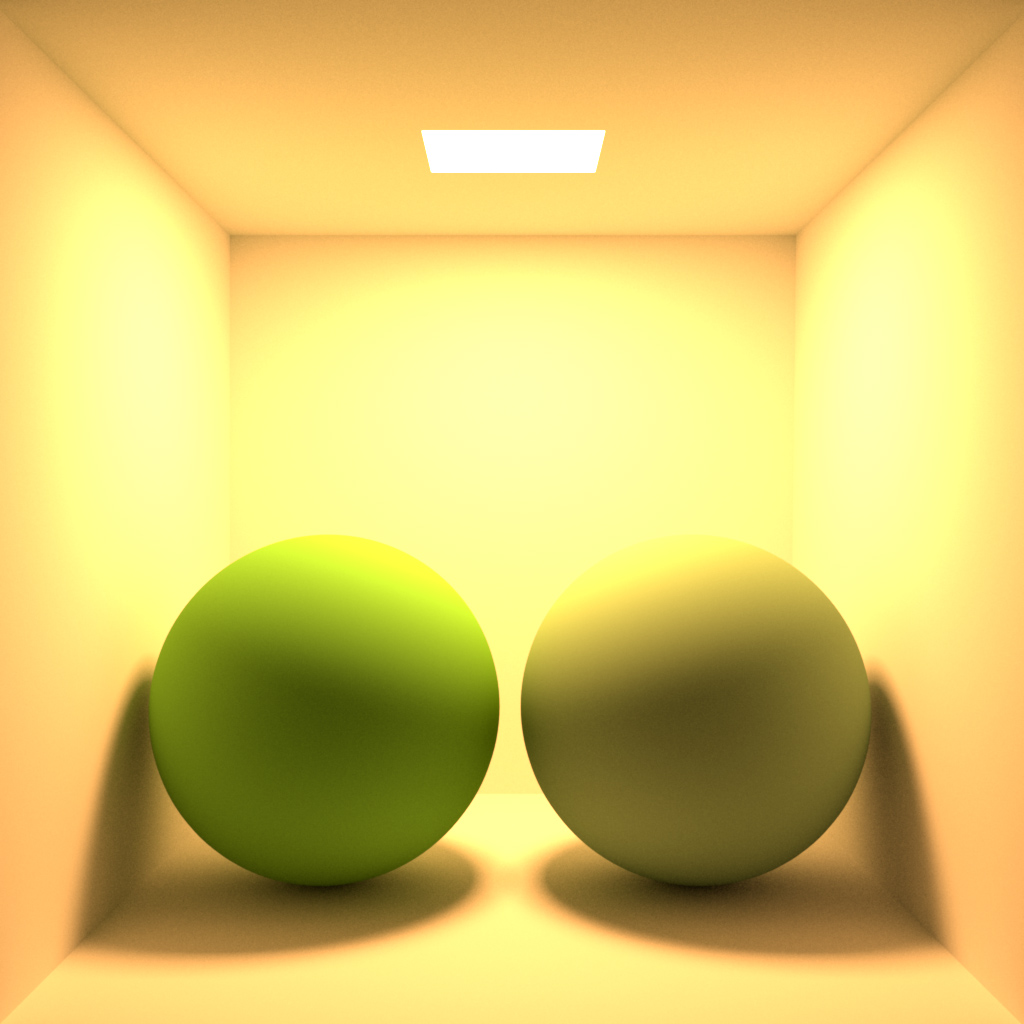
\includegraphics[alt={CIE Standard Illuminant A.},width=0.475\textwidth]{mitsuba-cornellbox-metamerism-A.jpg}
    \fi
    \ifdefined\HCode
        \ccJeriContainer{simple-jeri-embedding}
        \JavaScript
            const simpleJeriEmbeddingData = {
                title: 'Simple Jeri Embedding',
                children: [{
                        title: 'Illuminant E',
                        image: 'assets/images/mitsuba-cornellbox-metamerism-E.exr',
                    },
                    {
                        title: 'CIE Standard Illuminant A',
                        image: 'assets/images/mitsuba-cornellbox-metamerism-A.exr',
                    }
                ]
            };
            Jeri.renderViewer(document.getElementById('simple-jeri-embedding'), simpleJeriEmbeddingData);
        \EndJavaScript
    \fi
    \caption{
        Simple \textit{Jeri} Embedding.
    }
    \label{fig:simple-jeri-embedding}
\end{figure}
\end{lstlisting}

\begin{figure}[H]
    \unless\ifdefined\HCode
        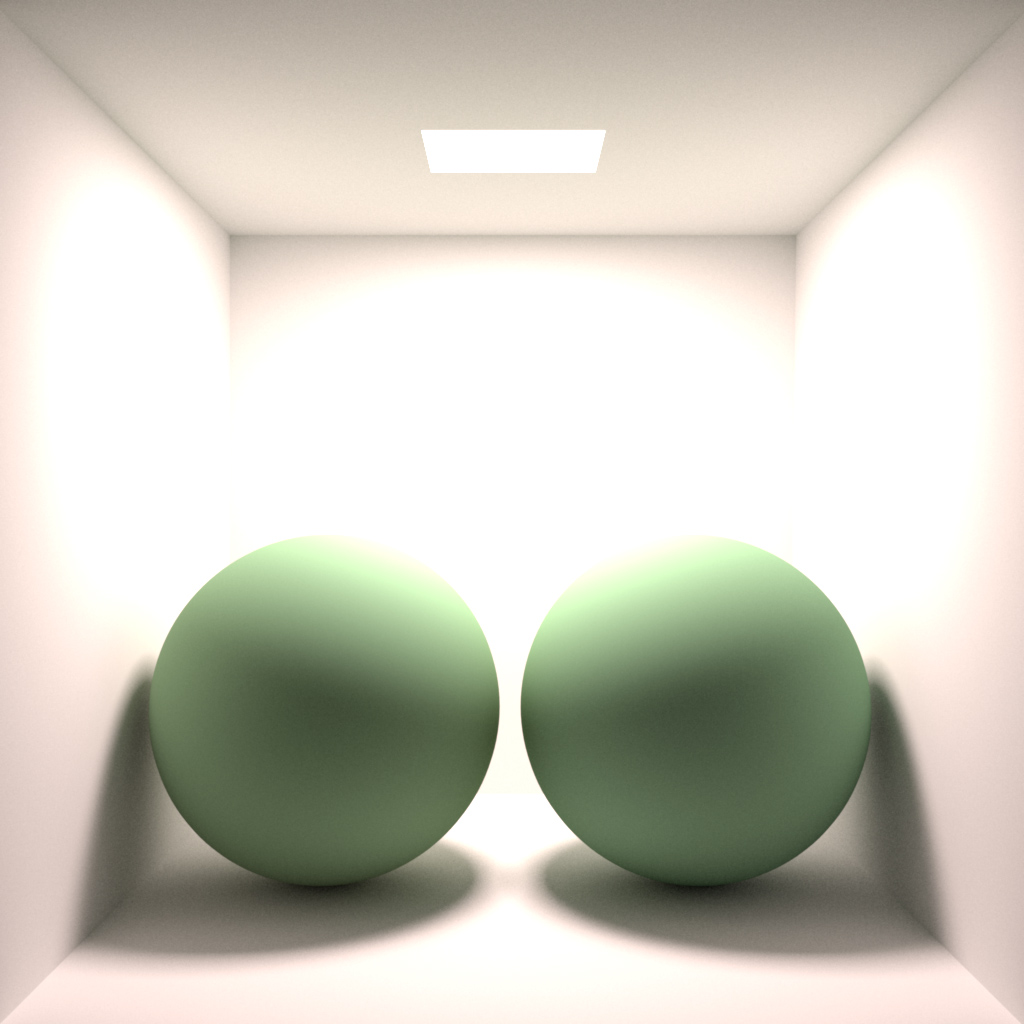
\includegraphics[alt={Illuminant E.},width=0.475\textwidth]{mitsuba-cornellbox-metamerism-E.jpg}\hfill
        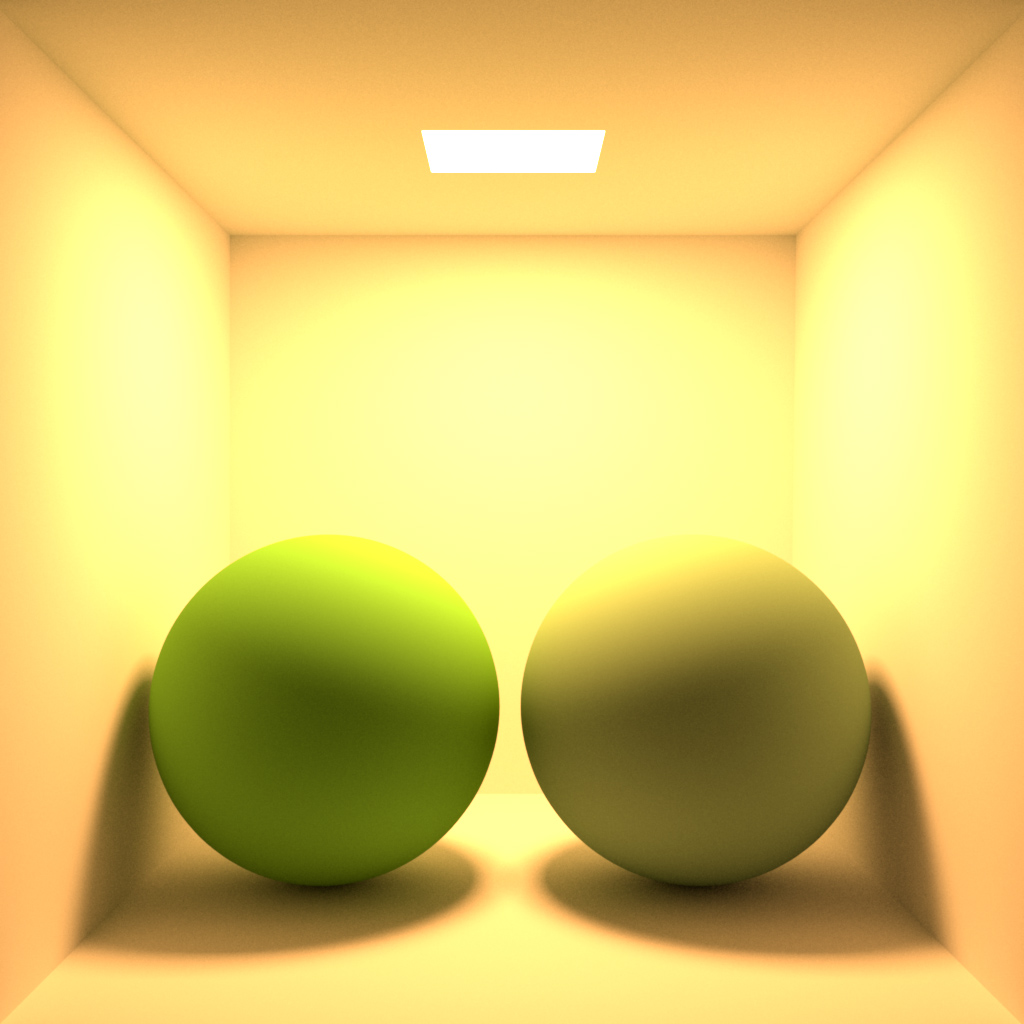
\includegraphics[alt={CIE Standard Illuminant A.},width=0.475\textwidth]{mitsuba-cornellbox-metamerism-A.jpg}
    \fi
    \ifdefined\HCode
        \ccJeriContainer{simple-jeri-embedding}
        \JavaScript
            const simpleJeriEmbeddingData = {
                title: 'Simple Jeri Embedding',
                children: [{
                        title: 'Illuminant E',
                        image: 'assets/images/mitsuba-cornellbox-metamerism-E.exr',
                    },
                    {
                        title: 'CIE Standard Illuminant A',
                        image: 'assets/images/mitsuba-cornellbox-metamerism-A.exr',
                    }
                ]
            };
            Jeri.renderViewer(document.getElementById('simple-jeri-embedding'), simpleJeriEmbeddingData);
        \EndJavaScript
    \fi
    \caption{
        Simple \textit{Jeri} Embedding.
    }
    \label{fig:simple-jeri-embedding}
\end{figure}

\subsection*{Complex Jeri Embedding}%

A complex \textit{Jeri} embedding example that only shows in the \textit{HTML}
output. The nested tab hierarchy has no elegant equivalent in the \textit{PDF}
output thus it not recommended to use nested tabs.

\begin{lstlisting}[caption={Complex \textit{Jeri} Embedding.}]
\begin{figure}[H]
    \ifdefined\HCode
        \ccJeriContainer{complex-jeri-embedding}
        \JavaScript
            const complexJeriEmbeddingData = {
                title: 'Complex Jeri Embedding',
                children: [{
                        title: 'Illuminant E',
                        image: 'assets/images/mitsuba-cornellbox-metamerism-E.exr',
                    },
                    {
                        title: 'CIE Standard Illuminant A',
                        image: 'assets/images/mitsuba-cornellbox-metamerism-A.exr',
                    },
                    {
                        title: 'Cornell Balls',
                        children: [{
                                title: 'Spectral',
                                image: 'assets/images/mitsuba-cornellbox-spectral.exr',
                            },
                            {
                                title: 'Sharp Primaries',
                                image: 'assets/images/mitsuba-cornellbox-sharp.exr',
                            }
                        ]
                    }
                ]
            };
            Jeri.renderViewer(document.getElementById('complex-jeri-embedding'), complexJeriEmbeddingData);
        \EndJavaScript
    \fi
    \caption{
        Complex \textit{Jeri} Embedding.
    }
    \label{fig:complex-jeri-embedding}
\end{figure}
\end{lstlisting}

\begin{figure}[H]
    \ifdefined\HCode
        \ccJeriContainer{complex-jeri-embedding}
        \JavaScript
            const complexJeriEmbeddingData = {
                title: 'Complex Jeri Embedding',
                children: [{
                        title: 'Illuminant E',
                        image: 'assets/images/mitsuba-cornellbox-metamerism-E.exr',
                    },
                    {
                        title: 'CIE Standard Illuminant A',
                        image: 'assets/images/mitsuba-cornellbox-metamerism-A.exr',
                    },
                    {
                        title: 'Cornell Balls',
                        children: [{
                                title: 'Spectral',
                                image: 'assets/images/mitsuba-cornellbox-spectral.exr',
                            },
                            {
                                title: 'Sharp Primaries',
                                image: 'assets/images/mitsuba-cornellbox-sharp.exr',
                            }
                        ]
                    }
                ]
            };
            Jeri.renderViewer(document.getElementById('complex-jeri-embedding'), complexJeriEmbeddingData);
        \EndJavaScript
    \fi
    \caption{
        Complex \textit{Jeri} Embedding.
    }
    \label{fig:complex-jeri-embedding}
\end{figure}

\section*{Interactive Figures}%
\label{sec:interactive-figures}

\subsection*{Colour Analysis Interactive Figure}%

An interactive figure rendered with
\href{https://github.com/colour-science/colour-analysis-three.js}{Colour Analysis}
and \href{https://github.com/mrdoob/three.js/}{Three.js}.

\begin{lstlisting}[caption={\textit{Colour Analysis} interactive figure.}]
\begin{figure}[H]
    \ifdefined\HCode
        \cccolouranalysiscontainer{gamutView1}
        \JavaScript
            var gamutViewSettings = {
                    scene: {
                        background: '#f8f9fa'
                    },
                    fog: {
                        color: '#f8f9fa',
                    },
                    grid: {
                        colorCenterLine: '#b5b5b5',
                        colorGrid: '#d5d5d5'
                    },
                    camera: {
                        position: { x: -1, y: 1, z: 1 },
                    },
            }

            var primaryColourspace = 'sRGB';

            // CIE 1931 2-Degree Standard Observer - Color Matching Functions
            var colourspaceModel = 'CIE XYZ';
            var gamutView1 = new ColourAnalysis.GamutView(
                document.getElementById('gamutView1'),
                {
                    ...{
                        primaryColourspace: primaryColourspace,
                        colourspaceModel: colourspaceModel,
                    },
                    ...gamutViewSettings
                }
            );
            gamutView1.addViewAxesVisual();
            gamutView1.addSpectralLocusVisual();
            gamutView1.animate();
        \EndJavaScript
    \fi
    \caption{
        \textit{Colour Analysis} interactive figure.
    }
    \label{fig:colour-analysis-interactive-figure}
\end{figure}
\end{lstlisting}

\begin{figure}[H]
    \ifdefined\HCode
        \cccolouranalysiscontainer{gamutView1}
        \JavaScript
            var gamutViewSettings = {
                    scene: {
                        background: '#f8f9fa'
                    },
                    fog: {
                        color: '#f8f9fa',
                    },
                    grid: {
                        colorCenterLine: '#b5b5b5',
                        colorGrid: '#d5d5d5'
                    },
                    camera: {
                        position: { x: -1, y: 1, z: 1 },
                    },
            }

            var primaryColourspace = 'sRGB';

            // CIE 1931 2-Degree Standard Observer - Color Matching Functions
            var colourspaceModel = 'CIE XYZ';
            var gamutView1 = new ColourAnalysis.GamutView(
                document.getElementById('gamutView1'),
                {
                    ...{
                        primaryColourspace: primaryColourspace,
                        colourspaceModel: colourspaceModel,
                    },
                    ...gamutViewSettings
                }
            );
            gamutView1.addViewAxesVisual();
            gamutView1.addSpectralLocusVisual();
            gamutView1.animate();
        \EndJavaScript
    \fi
    \caption{
        \textit{Colour Analysis} interactive figure.
    }
    \label{fig:colour-analysis-interactive-figure}
\end{figure}

\section*{References and Citations}%
\label{sec:references-and-citations}

The \href{https://ctan.org/pkg/biblatex-apa}{biblatex-apa Reference}
package is used for references and citations.

\subsection*{Citations}%
\label{subsec:citations}

\begin{lstlisting}[caption={Citation for Single Author.}]
\textcite{ARRI2012a}
\end{lstlisting}

\textcite{ARRI2012a}

\begin{lstlisting}[caption={Citation for Multiple Authors.}]
\textcite{ARRI2012a,Barlow1964}
\end{lstlisting}

\textcite{ARRI2012a,Barlow1964}

\subsection*{Citations with Parentheses}%
\label{subsec:citations-with-parentheses}

\begin{lstlisting}[caption={Citation with Parentheses for Single Author.}]
\parencite{ARRI2012a}
\end{lstlisting}

\parencite{ARRI2012a}

\begin{lstlisting}[caption={Citation with Parentheses for Multiple Authors.}s]
\parencite{ARRI2012a,Barlow1964}
\end{lstlisting}

\parencite{ARRI2012a,Barlow1964}
